\documentclass[12pt,a4paper]{article}

% Margins.
\setlength{\oddsidemargin}{0in}
\setlength{\evensidemargin}{0in}
\setlength{\headheight}{12pt}
\setlength{\headsep}{42pt}
\setlength{\topmargin}{-54pt}
\setlength{\textwidth}{6.5in}
\setlength{\textheight}{10in}

\usepackage{amsmath}
\usepackage{float}
\usepackage{graphicx}
\usepackage[hyphens]{url}
\usepackage{hyperref}	% Clickable links to figures, references and urls.
\usepackage{datetime}
\usepackage{longtable}
\usepackage{subfigure}

% Links direct to top of figures.
\usepackage[all]{hypcap}

% Drawing.
\usepackage{pgf}
\usepackage{tikz}

% Listings for formatting code.
\usepackage{listings}
\usepackage{textcomp}
% General options.+++
\lstset{breaklines=true, basicstyle=\small\ttfamily, tabsize=4, numbers=left, stepnumber=1, frame=single, showstringspaces=false, upquote=true}
% C++ specific high-lighting. Comments are 50/50 shades of green/black and strings coloured with 60/40 red/black mixture.
\lstset{language=[ISO]C++, commentstyle=\color{green!50!black}, keywordstyle=\color{blue}, stringstyle=\color{red!60!black}}

%opening
\title{\vspace{-3cm}Physics for Engineers\\Class 23\\Gauss's Law}
\author{Attique Dawood}
\date{October 09, 2013\\[0.2cm] Last Modified: \today, \currenttime}
\begin{document}
\maketitle
\section{Announcements}
\begin{itemize}
\item None.
\end{itemize}
\section{Revision}
\begin{itemize}
\item Electric field lines.
\item Motion of a charged particle in uniform electric field.
\end{itemize}
\section{Gauss's Law}
Gauss's Law is one of the four fundamental equations of electromagnetics also known as Maxwell's equations. Suppose there is an electric field in a region. Pick any imaginary closed surface. \textbf{The total electric flux through any closed surface is equal to $\dfrac{1}{\epsilon_0}$ times the total charge enclosed by the surface}. Mathematically
\begin{equation}
\oint_{S}\textbf{E}\cdot d\textbf{S}=\dfrac{q}{\epsilon_0}.
\end{equation}
A closed surface always encloses a volume and we're interested in the total charge within the volume. Note that \textbf{E} and d\textbf{S} are \textbf{on} the closed surface. Also note that d\textbf{S} is normal vector on the surface. \textbf{Solving the integral is easiest when electric field is also perpendicular to the surface} because then the magnitudes of electric field and differential surface can be simply multiplied. Further to this if the electric field is uniform over (or on) the entire surface then it can be taken out of the integral reducing the integral to
\begin{equation}
E\oint_{S}dS=\dfrac{q}{\epsilon_0}.
\end{equation}
Left hand side is simply magnitude of \textbf{E} multiplied with the total surface area. \textbf{Gauss's Law can be used to find unknown electric field if we know the direction of electric field}.
\begin{equation}
\begin{split}
&E\oint_{S}dS=\dfrac{q}{\epsilon_0}\\
&EA=\dfrac{q}{\epsilon_0}\\
&E=\dfrac{q}{\epsilon_0A}.
\end{split}
\end{equation}
\section{Exercises}
\noindent\textbf{Question 1:} Use Gauss's Law to find electric field of a point charge.\\[0.2cm]
\noindent\textbf{Question 2:} Electric field in a region is $\textbf{E}=y\hat y$. Find the total charge enclosed in a unit cube defined by $1<y<2$, $0<x<1$ and $0<z<1$.
%\begin{itemize}
%\item[a.] Electric field of a point charge.
%\item[b.] Electric field of an infinite line charge placed along $z$--axis.
%\end{itemize}
%%\begin{figure}[H]
%\centering
%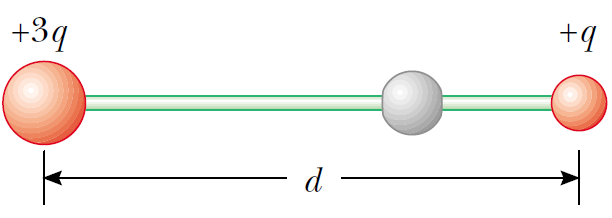
\includegraphics[scale=0.45]{FigureP23-10.png}
%\caption{Equilibrium of charge.}
%\label{Equilibrium}
%\end{figure}
%\nocite{*}
%\bibliographystyle{plain}
%\bibliography{PhysicsRef}
\end{document}
